\documentclass[sokoban_generation_thesis.tex]{subfiles}
Metoda SYM opiera swoje działanie na~decyzjach agenta, które podejmowane są~zgodnie ze~strategiami opisanymi w~p.~\ref{sub:sym_strategie}. Eksperymenty, których wyniki opisano w~tym podrozdziale, zostały wykonane dla każdej z~$72$ możliwych konfiguracji strategii, a~następnie uśrednione.


\subsection{Wydajność czasowa} \label{subs:sym_time}
W celu zbadania wydajności czasowej metody SYM, wykonano eksperyment badający średni czas wykonania zadanej liczby iteracji \textit{forward} oraz \textit{backward}. W~eksperymencie uwzględniono wszystkie możliwe konfiguracje strategii oraz rozmiary plansz z~zakresu $[5,30]$. Wyniki analizy, ukazane na~rys.~\ref{rys:sym_its_czas}, wykazały iż~średnio rozgrywka \textit{forward} nie trwała dłużej niż $0.25$ sekundy, a~rozgrywka \textit{backward} -- $0.1$ sekundy. Co~więcej, dla liczby iteracji poniżej stu, generacja planszy zajmowała średnio mniej niż $0.122$ sekundy.

\begin{figure}[h!]
	\centering
	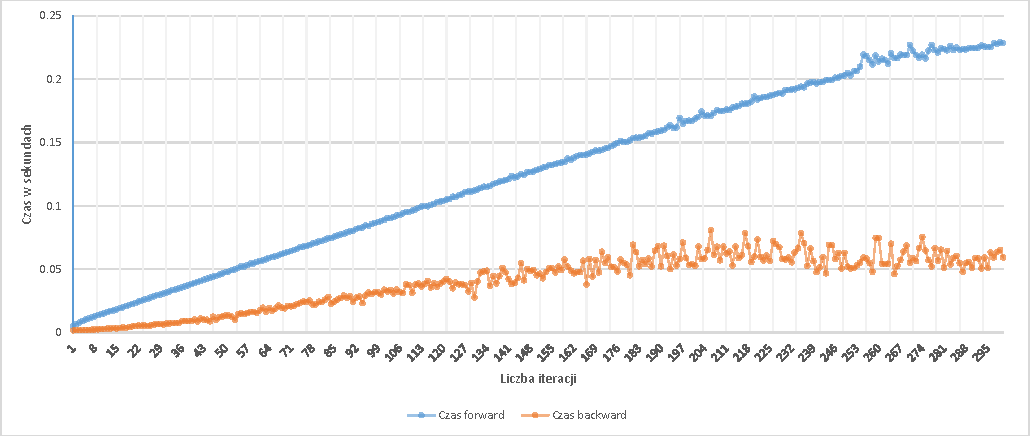
\includegraphics[width=0.92\textwidth]{wykres_sym_czas_iteracji}
	\caption{Zależność czasu od~liczby iteracji}
	\label{rys:sym_its_czas}
\end{figure}

Autorzy metody SYM zestawiają wydajność czasową swojej metody z~innym algorytmem \cite{heur_worse}, który również jest metodą heurystyczną symulującą rozgrywkę. Metoda SYM wygrywa ze~swoim odpowiednikiem przede wszystkim ze~względu na~niezależność od~liczby pudeł na~generowanej planszy. Metoda \cite{heur_worse} dla liczby pudeł poniżej sześciu uzyskuje podobne wyniki, za~to~zależność czasu od~liczby pudeł powyżej sześciu ma~charakter wykładniczy. Co~więcej, czas obliczeń odpowiednika metody SYM rośnie kwadratowo w~zależności od~wartości hiperparametru definiującego skomplikowanie plansz, czego nie obserwuje się w~przypadku metody SYM. Wnioskuj się, iż~jest to~najbardziej wydajna czasowo opublikowana metoda heurystyczna generowania plansz \textit{Sokoban} \cite{heur_sim}.

\subsection{Liczba iteracji}
\begin{figure}[h!]
	\centering
	\begin{subfigure}[b]{0.27\textwidth}
		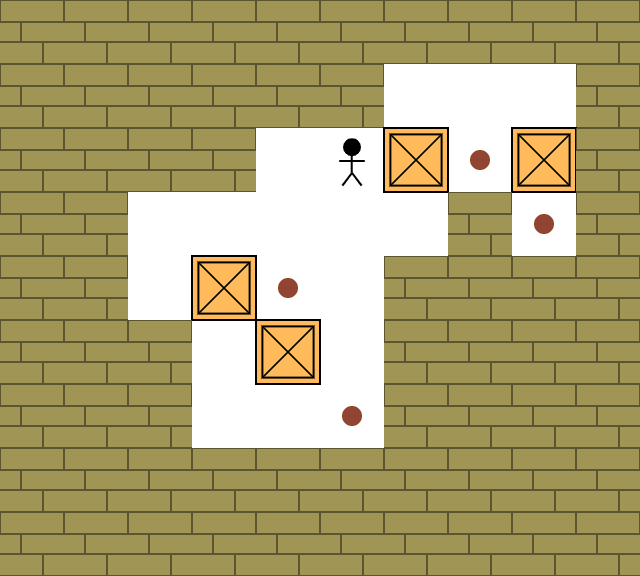
\includegraphics[width=\textwidth]{board_sym_step1}
		\caption{Plansza po~$4$ iteracjach}
	\end{subfigure}
	\hspace{0.04\textwidth}
	\begin{subfigure}[b]{0.27\textwidth}
		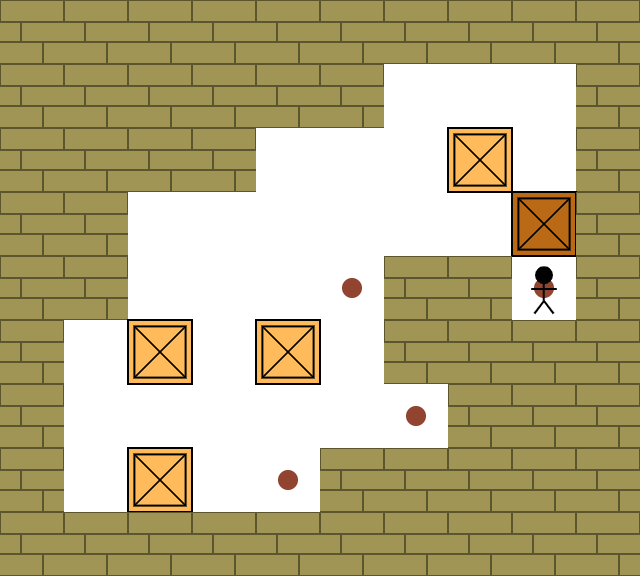
\includegraphics[width=\textwidth]{board_sym_step2}
		\caption{Plansza po~$10$ iteracjach}
	\end{subfigure}
	\hspace{0.04\textwidth}
	\begin{subfigure}[b]{0.27\textwidth}
		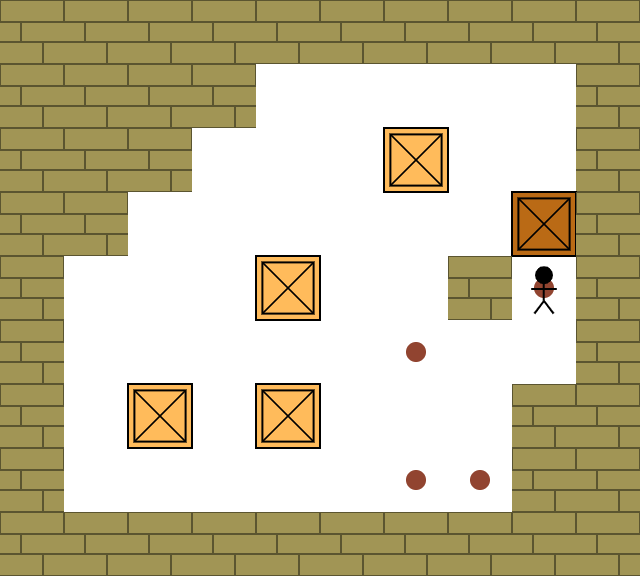
\includegraphics[width=\textwidth]{board_sym_step3}
		\caption{Plansza po~$30$ iteracjach}
	\end{subfigure}
	\caption{Wpływ liczby iteracji \textit{forward} na~wypełnienie generowanych plansz}
	\label{rys:sym_dodawanie_f}
\end{figure}

Wraz ze~zwiększaniem liczby iteracji \textit{forward} w~metodzie SYM, plansze zyskują coraz więcej pustych pól, co~można zaobserwować na~rys.~\ref{rys:sym_dodawanie_f}. To~oznacza, że~zmniejsza się ich wypełnienie -- stosunek niepustych pól do~wszystkich pól na~planszy. Sugeruje się, że~większość istotnie skomplikowanych plansz charakteryzuje się wypełnieniem na~poziomie od~$50\%$ do~$55\%$ \cite{sok_metrics2}. Aby sprawdzić charakter wypełnienia dla analizowanej metody, dokonano generacji $5000$ plansz rozmiaru $8x8$ z~użyciem różnych kombinacji parametrów, dla określonego zakresu liczby iteracji \textit{forward} i~\textit{backward}. Wyniki analizy zaprezentowano na~rys.~\ref{rys:sym_its_wypelnienie}. Jak widać, dla tego rozmiaru planszy, żądane wypełnienie uzyskuje się dla liczby iteracji \textit{forward} z~zakresu $[17, 30]$. Liczba iteracji \textit{backward} nie ma~istotnego wpływu na~wypełnienie generowanych plansz.

\begin{figure}[h!]
	\centering
	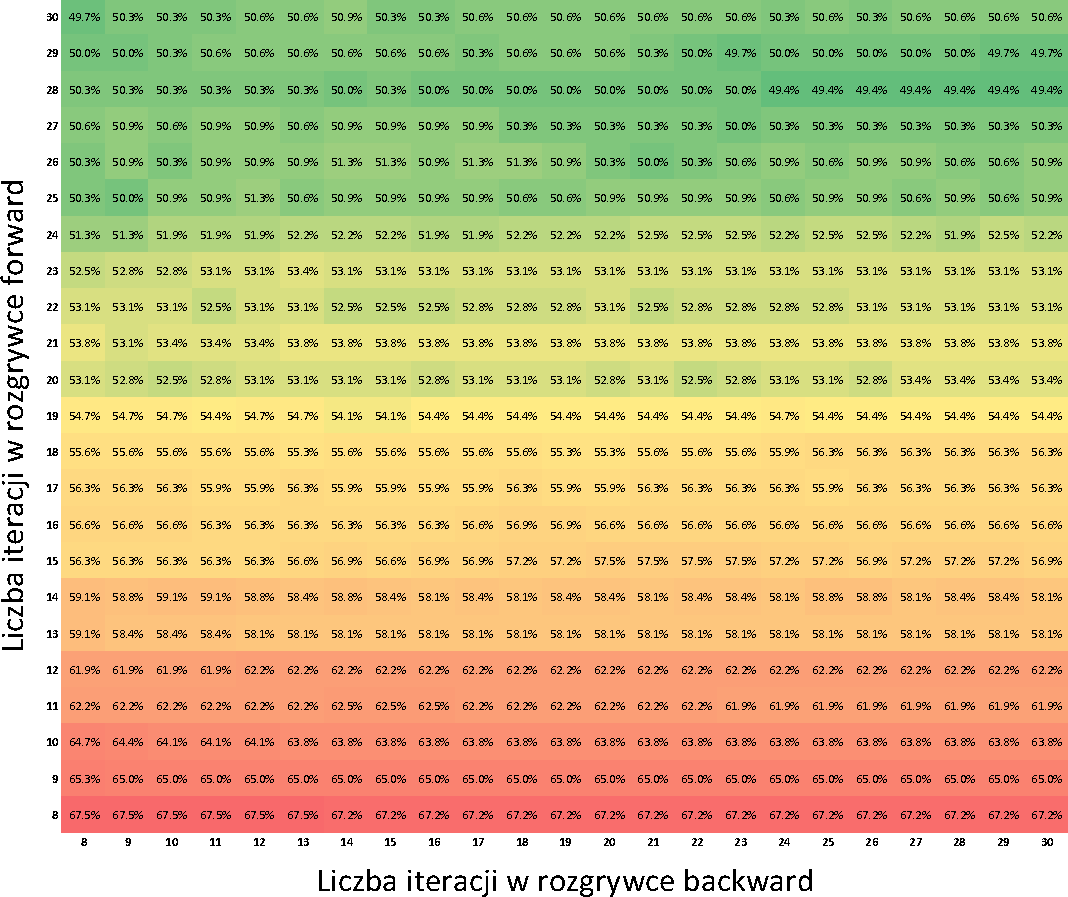
\includegraphics[width=0.7\textwidth]{wykres_sym_wypelnienie}
	\caption{Zależność wypełnienia generowanych plansz od~liczby iteracji}
	\label{rys:sym_its_wypelnienie}
\end{figure}

Jako że~samo wypełnienie nie jest gwarantem skomplikowania poziomów, postanowiono zbadać również zależność średniej sumy odległości pudeł od~ich pól docelowych. Owe odległości są~wyznaczone w~oparciu o~rozwiązania dostarczane przez samą metodę, co~oznacza że~nie muszą być najbardziej optymalne. Tym niemniej, wykonano eksperyment analogiczny do~poprzedniego, a~jego wyniki zaprezentowano na~rys.~\ref{rys:sym_its_odleglosci}. Jak widać, niezależnie od~użytej liczby iteracji \textit{forward}, wraz ze~wzrostem liczby iteracji \textit{backward}, sumy odległości rosły, czyniąc plansze bardziej skomplikowanymi. Dla niektórych przypadków, zwiększenie liczby iteracji \textit{backward} wydłużało sumę odległości o~ponad $40\%$.

\begin{figure}[h!]
	\centering
	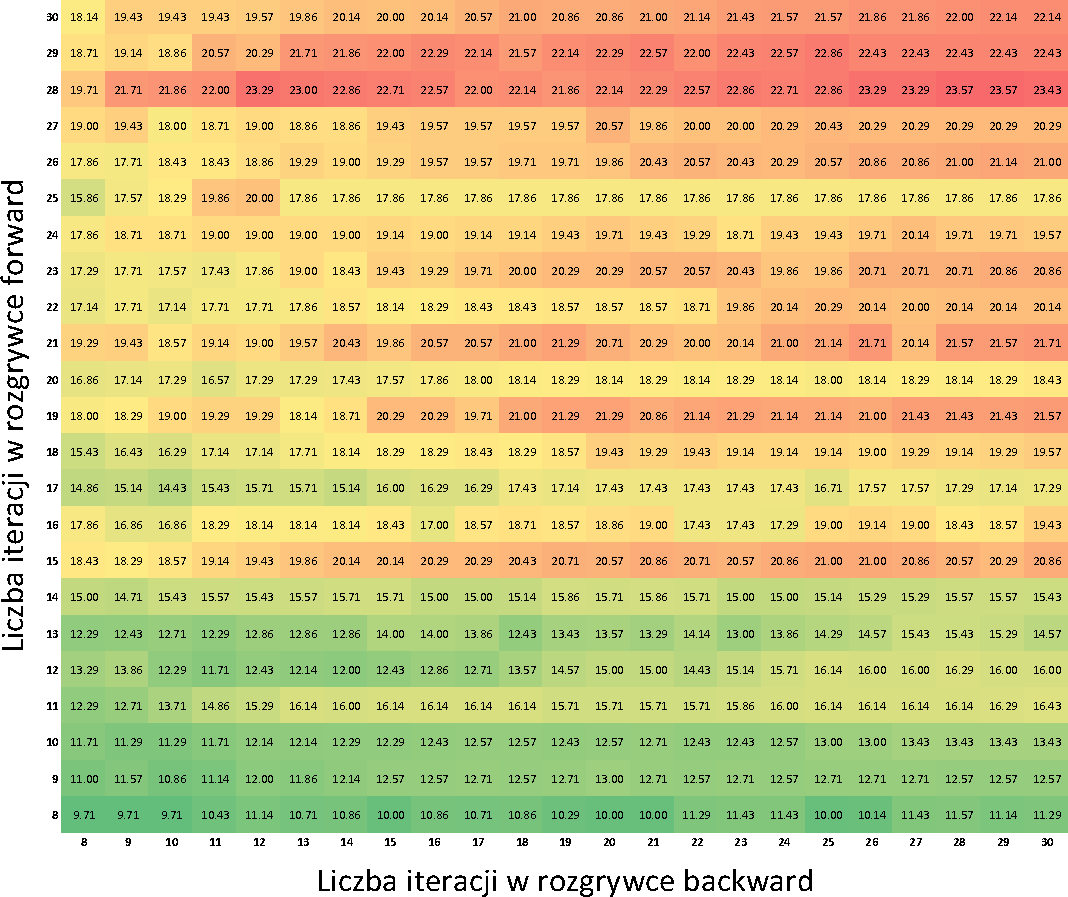
\includegraphics[width=0.7\textwidth]{wykres_sym_odleglosc}
	\caption{Zależność sumy odległości między pudłami a~polami docelowymi od~liczby iteracji}
	\label{rys:sym_its_odleglosci}
\end{figure}
